\chapter{Package MARSS:  The top-level MARSS functions and the base functions}

Package MARSS includes functions for estimating Multivariate Autoregressive State Space models, obtaining confidence intervals for parameters, and calculating Akaike's Information Criterion (AIC) for model selection.  To make the package both flexible and easy to use, it is designed in two levels.  At the base level, the programmer can interact directly with the estimation functions, using two kinds of R objects:  objects of the model specification class `marssm', and objects of estimation classes such as `marssMLE'.  At the user level, the \verb@MARSS()@ function allows model estimation with just one function call, hiding the details for ease of use.  Users create models in an intuitive way by specifying constraints; the \verb@MARSS()@ function then converts these constraints into the object structures required by the estimation functions, performing error checking as necessary.

The two-level package structure allows new users convenient access to the underlying functions, while maintaining flexibility to incorporate different applications and algorithms.  Developers can use the base object types to write new functions for their own modeling applications. 

To use \verb@MARSS()@, the user specifies a model by supplying the constraint argument to  \verb@MARSS()@, using the method argument to specify an estimation method.  Optionally, the user may provide initial values for the free parameters, and specify estimation options; for details see the  \verb@MARSS()@ help file.  The function returns an object containing the model, parameter values and estimation details.  The user may pass the returned object to  \verb@MARSSboot()@, which generates bootstrap parameter estimates, or to  \verb@MARSSaic()@, which calculates various versions of AIC for model selection.

Figure C.1 shows the underlying base level operations \verb@MARSS()@ performs.  The function creates a wrapper object of class `popWrap'.  It then calls the \verb@as.marssm()@ method for `popWrap' to create a marssm object from the constraints provided.  This model object, initial values and control information are the minimal information required by the estimation functions, and are combined into an object of class appropriate for the estimation method.  The estimation function adds to this object the estimated parameter values, estimation details, and other function-specific components, and then returns the augmented object.

\begin{figure}[htp]
\begin{center}
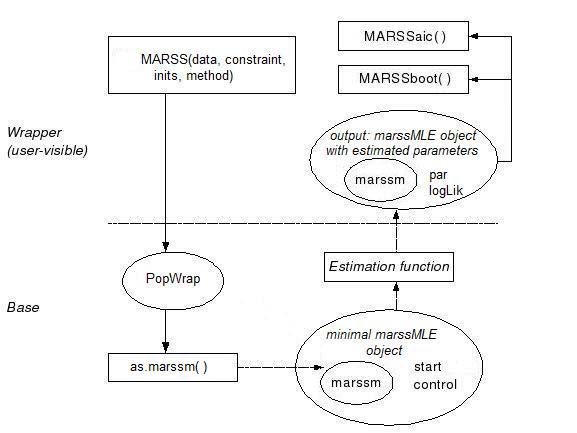
\includegraphics{../figures/Fig1}
\end{center}
\caption{Two-level structure of the MARSS package.  Rectangles represent functions; ovals represent objects.}
\end{figure}

